\chapter{Подходы к решению задачи Person Re-Id}
\label{ch:closed-world}

 Общая схема построения работы системы идентификации людей содержит следующие этапы:

 \begin{enumerate}
     \item Обучение представлений признаков

     \item Метрическое обучение

     \item Оптимизация ранжирования.
    
 \end{enumerate}

 Обучение представлений признаков, или feature representation learning, $-$ это этап, на котором применяется какая-либо модель машинного обучения, позволяющая эффективно преобразовывать входное изображение в векторное представление $-$ \textit{эмбеддинг}. Данное векторное представление должно быть достаточно репрезентативным, чтобы предоставлять возможность определять по нему похожесть изображений $-$ степень уверенности в том, что на них представлен один и тот же человек. 

 Для выполнения этих требований применяются техники глубокого метрического обучения (deep metric learning). Они повзоляют построить эмбеддинги в \textit{метрическом пространстве}, то есть наделить их пространство функцией расстояния. В таком случае возникает возможность сравнивать представления изображений по их близости. Исходя из близости эмбеддингов изображений, могут быть получены ранжированние списки для изображений-запросов. Они получаются путем сортировки всех изображений из базы согласно близости их векторных представлений к эмбеддингу запроса.

 Затем, когда получены ранжированные списки, могут быть применены специальные подходы их оптимизации. Эти подходы заключаются в сравнении различных ранжированных списков между собой, для выявления более четких взаимосвязей между данными.

 Далее рассмотрим подробнее каждый этап работы системы и применяемые техники; обсудим, какие из них показывают наилучшие результаты на данный момент.


 \section{Обучение представлению признаков}

 Существует множество подходов, направленных на то, чтобы сделать эмбеддинг изображения наиболее информативным. На \hyperref[fig:feat_repr]{Рисунке \ref*{fig:feat_repr}} проиллюстрированы основные различия в этих подходах. Во-первых, базовый вариант $-$ подавать изображение напрямую в модель компьютерного зрения: сверточную сеть или трансформер, $-$ для получения итогового эмбеддинга. Во-вторых, некоторые подходы используют разделение кадра на смысловые части, позволяющее учесть локальные признаки, соответствующие, например, определенным частям тела. В-третьих, существует подходы, которые прибегают к вспомогательной информации для наделения эмбеддинга изображения дополнительными свойствами. И, наконец, часть подходов опирается на тот факт, что все кадры, содержащие целевой объект, поступают на вход системы из видеозаписи, что позволяет обрабатывать их как упорядоченную последовательность и моделировать более состоятельные закономерности.

 \begin{figure}[ht]
     \centering
     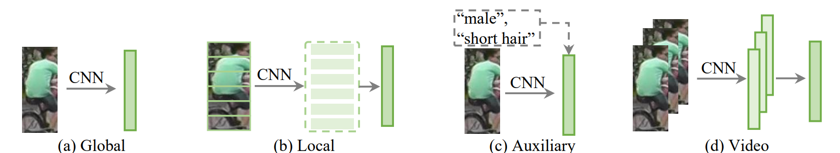
\includegraphics{images/closed_world/feat_repr_learning.png}
     \caption{Варианты работы системы на этапе обучения представлению признаков \cite{ye2021deep}}
     \label{fig:feat_repr}
 \end{figure}

 \subsection{Глобальное представление признаков}

 Данный вариант представляет собой применение, или \textit{инференс}, нейросети компьютерного зрения на изображении целиком. Так, сверточная сеть, преобразует входной кадр на каждом слое в карту признаков, из которой в итоге формируется один эмбеддинг. В базовом случае этот процесс применяется к каждому изображению датасета в режиме \textit{single-image}, то есть независимо. Однако существуют методы, которые принимают на вход пары изображений, что соответствует режиму \textit{cross-image} \cite{wang2016joint}. В таком случае карты признаков обоих изображений подаются вместе в модель построения итогового эмбеддинга, как показано на \hyperref[fig:cross_image]{Рисунке \ref*{fig:cross_image}}. Таким образом система работает в режиме верификации $-$ определения того, соответствуют два изображения одному и тому же человеку или нет.

 \begin{figure}[ht]
     \centering
     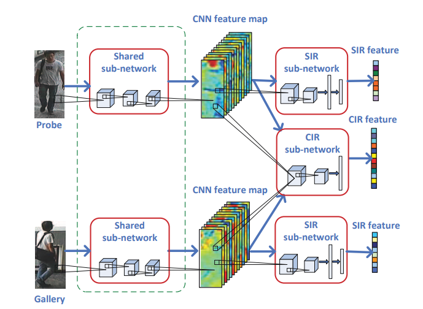
\includegraphics[width=0.7\textwidth]{images/closed_world/single_cross_image.png}
     \caption{Single-image и Cross-image режимы \cite{wang2016joint}}
     \label{fig:cross_image}
 \end{figure}

 \subsection{Локальное представление признаков}

 Методы этого типа раскладывают входное изображение на несколько пространственных составляющих, отвечающих различным \textit{регионам интереса}. Во-первых, регионы интереса могут соответствовать частям тела и использовать отдельную модель детекции для определения их местоположения \cite{suh2018part}, как показано на \hyperref[fig:body_part]{Рисунке \ref*{fig:body_part}}.

 \begin{figure}[ht]
     \centering
     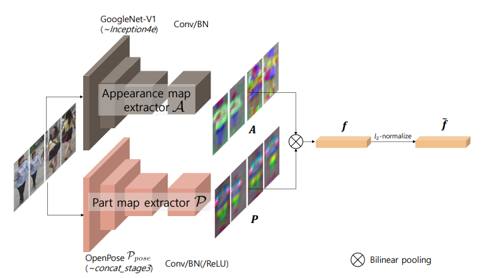
\includegraphics[width=0.7\textwidth]{images/closed_world/body_part_detection.png}
     \caption{Извлечение локальных признаков с помощью детекции частей тела \cite{suh2018part}}
     \label{fig:body_part}
 \end{figure}

 Во-вторых, некоторые методы \cite{su2018beyond} обрабатывают регионы интереса как отдельные изображения, что позволяет параллельно извлечь из кадра информацию разного типа. При этом регионы могут быть получены исходя из детекции частей тела, ключевых точек или же из нарезки изображения на равные слои по вертикали или по горизонтали (см. \hyperref[fig:image_slicing]{Рисунок \ref*{fig:image_slicing}}).

 \begin{figure}[ht]
     \centering
     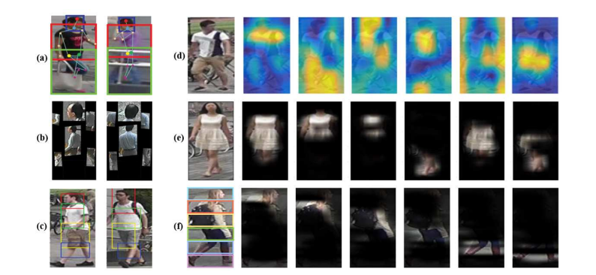
\includegraphics[width=0.7\textwidth]{images/closed_world/image_slicing.png}
     \caption{Нарезка изображения на части \cite{su2018beyond}}
     \label{fig:image_slicing}
 \end{figure}

 \subsection{Использование дополнительной информации}

 Наибольший научный интерес в рамках данной работы представляют методы, прибегающие к вспомогательной информации для построения информативного эмбеддинга изображения человека. 

 Одна группа таких методов опирается на семантические атрибуты $-$ текстовые описания или же метки классификации \cite{lin2019improving}, \hyperref[fig:semantic_attributes]{Рисунок \ref*{fig:semantic_attributes}}. Действительно, каждый человек в рамках данной задачи может быть классифицирован по таким категориям, как пол, возраст, цвет и длина волос, тип и цвет одежды и др. Информация об этой классификации может подаваться в модель в разном виде. Она может подаваться на вход, может сроиться отдельный эмбеддинг модели классификации. Также с помощью дополнительной инфорации может строиться фильтрация релевантных/не-релевантных объектов. Кроме того, могут применяться метрические методы для установления соответствия между эмбеддингом атрибутной информации и основным эмбеддингом изображения.

 \begin{figure}[ht]
     \centering
     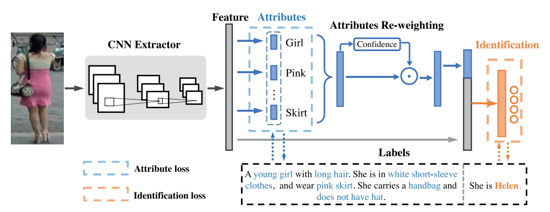
\includegraphics[width=0.7\textwidth]{images/closed_world/semantic_attributes.png}
     \caption{Использование семантических атрибутов \cite{lin2019improving}}
     \label{fig:semantic_attributes}
 \end{figure}

 Также существует методы, рассматривающие изображения с каждой камеры как отдельный домен, то есть однородную часть в неоднородном общем датасете \cite{liu2019view}, \hyperref[fig:viewpoint_information]{Рисунок \ref*{fig:viewpoint_information}}.

 \begin{figure}[ht]
     \centering
     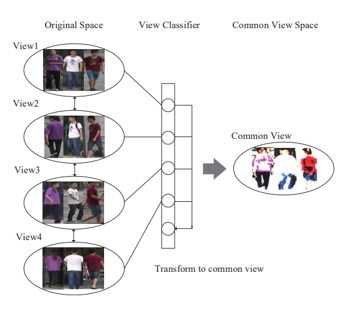
\includegraphics[width=0.5\textwidth]{images/closed_world/viewpoint_information.png}
     \caption{Кросс-доменная идентификация для кадров с различных камер \cite{liu2019view}}
     \label{fig:viewpoint_information}
 \end{figure}

 В такой постановке применяются технологии кросс-доменной идентификации, направленные на построения таких представлений изображений, которые обладают инвариантностью к смене домена. Так, например, один из методов включает в функцию потерь ограничение на близость между матрицами корреляций признаков изображений из разных доменов \cite{lin2017consistent}, \hyperref[fig:domain_information]{Рисунок \ref*{fig:domain_information}}.

 \begin{figure}[ht]
     \centering
     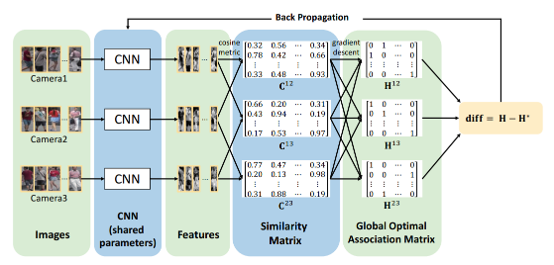
\includegraphics[width=0.7\textwidth]{images/closed_world/domain_information.png}
     \caption{Использование доменной информации \cite{lin2017consistent}}
     \label{fig:domain_information}
 \end{figure}

 Еще одной из важных техник, затрагивающей дополнительную информацию, является аугментация датасетов, в том числе с помощью генеративных моделей \cite{zheng2017unlabeled}. Общий план такого метода, как показано на \hyperref[fig:dataset_augmentation]{Рисунке \ref*{fig:dataset_augmentation}}, состоит в том, чтобы дополнить датасет данными для тех объектов, для которых мало размеченных примеров, и использовать полученные синтетические данные при обучения модели.

 \begin{figure}[ht]
     \centering
     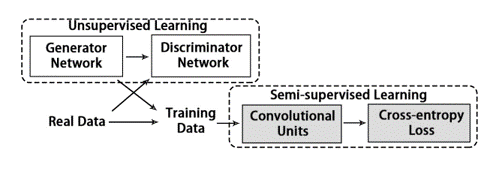
\includegraphics[width=0.5\textwidth]{images/closed_world/dataset_augmentation.png}
     \caption{Аугментация датасета с помощью генеративных моделей \cite{zheng2017unlabeled}}
     \label{fig:dataset_augmentation}
 \end{figure}

 \subsection{Идентификация на видео}

 Наконец, еще один способ промоделировать общие закономерности данных заключается в том, чтобы подавать кадры видеозаписей не по-отдельности, а в виде упорядоченной последовательности, что иллюстрирует \hyperref[fig:rnn]{Рисунок \ref*{fig:rnn}}. В таком случае применимы различные методы обработки последовательных данных, такие как рекуррентные сети и трансформеры \cite{haque2016recurrent}.

 \begin{figure}[ht]
     \centering
     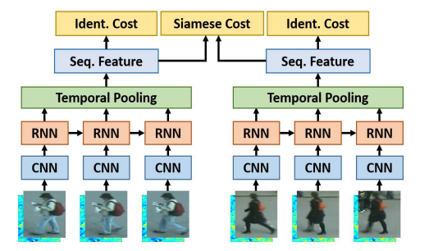
\includegraphics[width=0.5\textwidth]{images/closed_world/rnn.png}
     \caption{Применение моделей обработки последовательностей для видео \cite{haque2016recurrent}}
     \label{fig:rnn}
 \end{figure}



 \section{Метрическое обучение}

 Ключевая часть в построении системы, решающей задачу \reid\ $-$ это метрическое обучение, или \textit{metric learning}. Его суть состоит в том, чтобы с помощью функции потерь учесть тот факт, что эмбеддинги должны лежать в метрическом пространстве. Таким образом, эмбеддинги кадров, соответствующих одному и тому же человеку, должны лежать близко к друг другу, а между изображениями разных людей расстояние должно быть большим. В такой постановке возникает два важных аспекта работы $-$ дизайн самой лосс-функции и построение хода обучения таким образом, чтобы на каждой итерации модель с помощью этой лосс-функции усваивала наиболее важные закономерности в данных.

 \subsection{Дизайн функции потерь}

 \textbf{Softmax loss}. Базовый вариант $-$ обучение модели на решение задачи классификации. В таком случае каждый класс $-$ это один человек, представленный в датасете, и модель обучается отличать их друг от друга, используя softmax loss, или же identity loss, \hyperref[fig:identity_loss]{Рисунок \ref*{fig:identity_loss}}:

 \begin{figure}[ht]
     \centering
     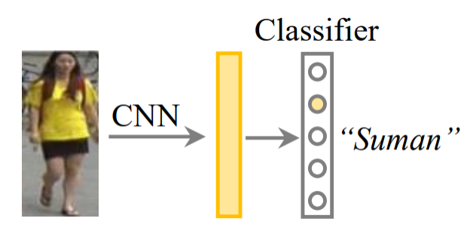
\includegraphics[width=0.5\textwidth]{images/closed_world/identity_loss.png}
     \caption{Лосс-функция идентификации \cite{ye2021deep}}
     \label{fig:identity_loss}
 \end{figure}

 \begin{equation}
     \mathcal L_{S} = \mathcal L_{id} = - \frac{1}{n}\sum \limits_{i = 1}^n \log \left( p (y_i | x_i) \right) = \frac{1}{n}\sum \limits_{i = 1}^n \log \frac{e^{W_{y_i}^T x_i + b_{y_i}}}{\sum_{j=1}^m e^{W_j^T x_i + b_j}}.
 \end{equation}

 Здесь $n$ $-$ количество объектов в батче, $m = |Search|$ $-$ количество классов, то есть различных людей в датасете, $x_i$ $-$ эмбеддинг $i$-того объекта, $W_j$ и $b_j$ $-$ вес и свободный член классификатора, соответстующие данному классу $j$.

 Недостаток этого метода состоит в том, что нет гарантий для применимости этого метода для неизвестных объектов, поскольку свойство метрического пространства не закладывается в модель.

 \textbf{Center loss}. Один из вариантов наделения пространства эмбеддингов информативной метрикой $-$ кластеризация \cite{wen2016discriminative}, \hyperref[fig:center_loss]{Рисунок \ref*{fig:center_loss}}. Так, подход center loss заключается в том, чтобы добавить слагаемое, отвечающее за разделение эмбеддингов разных классов на кластеры:

 \begin{figure}[ht]
     \centering
     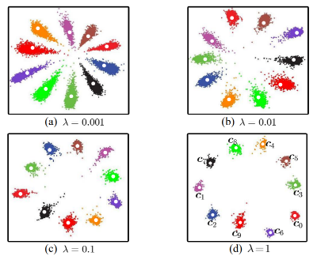
\includegraphics[width=0.5\textwidth]{images/closed_world/center_loss.png}
     \caption{Кластеризация с помощью center loss \cite{wen2016discriminative}}
     \label{fig:center_loss}
 \end{figure}

 \begin{equation}
     \mathcal L_{C} = - \frac{1}{2}\sum \limits_{i = 1}^n  \| x_i - c_{y_i} \|^2,
 \end{equation}
 \begin{equation}
     \mathcal L = \mathcal L_S + \lambda \mathcal L_C.
 \end{equation}

 \textbf{Binary verification loss}. В этом подходе изображения подаются в нейросеть парами. Для обоих изображений модель строить свой эмбеддинг, и затем эта пара эмбеддингов подается в итоговый бинарный классификатор: один и тот же это объект или нет \cite{li2014deepreid}, \hyperref[fig:binary_verification_loss]{Рисунок \ref*{fig:binary_verification_loss}}.

 \begin{figure}[ht]
     \centering
     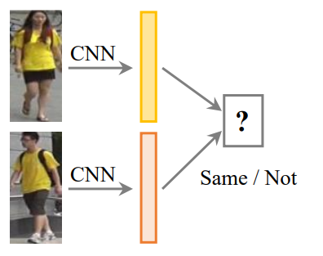
\includegraphics[width=0.5\textwidth]{images/closed_world/binary_verification_loss.png}
     \caption{Лосс-функция верификации \cite{li2014deepreid}, \cite{ye2021deep}}
     \label{fig:binary_verification_loss}
 \end{figure}

 \begin{equation}
     \mathcal L_{very}(i, j) = - \delta_{ij} \log \left( p(\delta_{ij} | x_{ij}) \right) - (1 - \delta_{ij}) \log \left( 1 - p(\delta_{ij} | x_{ij}) \right).
 \end{equation}

 Здесь $\delta_{ij}$ $-$ индикатор того, что кадры $i$ и $j$ представляют один объект, $x_{ij}$ $-$ их совместное представление. Недостаток этого метода состоит в том, что необходимо подавать изображения парами, следовательно, для поиска целевого объекта нужно перебрать все изображения из базы.

 \textbf{Contrastive loss}. В данном варианте можно подавать изображения в модель как парами, так и независимо. Лосс-функция накладывает на эмбеддинги свойства метрического пространства, пропорционально штрафуя модель за близкие по метрике $d$ представления изображений разных объектов и далекие представления разных \cite{hadsell2006dimensionality}. При этом используется пороговое значение отступа $\rho$, которое принимается достаточным для разделения объектов; выше этого значения штраф не назначается:

 \begin{equation}
     \mathcal L_{con} = (1 - \delta_{ij}) \{ \max (0, \rho - d_{ij}) \}^2 + \delta_{ij} d_{ij}^2.
 \end{equation}

 \textbf{Triplet loss}. Один из наиболее распространеных и эффективных методов является использование triplet loss-а \cite{schroff2015facenet}. Этот способ позволяет промоделировать более широкие взаимосвязи между данными. Изображения объединяются в тройки, содержащие опорный, или \textit{якорный}, объект, а также \textit{позитивный} и \textit{негативный} примеры. Позитивный пример соответствует тому же человеку, что и якорный, а негативный $-$ другому. Цель состоит в том, чтобы на очередном шаге оптимизации приблизить к опорному объекту $i$ позитивный пример $j$ и отдалить негативный $k$, \hyperref[fig:triplet_loss]{Рисунок \ref*{fig:triplet_loss}}.

 \begin{figure}[ht]
     \centering
     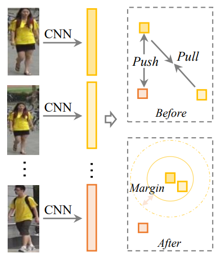
\includegraphics[width=0.5\textwidth]{images/closed_world/triplet_loss.png}
     \caption{Triplet loss \cite{schroff2015facenet}, \cite{ye2021deep}}
     \label{fig:triplet_loss}
 \end{figure}

 \begin{equation}
     \mathcal L_{tri} (i, j ,k) = \max \left( \rho + d_{ij} - d_{ik}, 0 \right).
 \end{equation}

 \textbf{SphereFace}. Этот метод представляет собой развитие softmax loss-а. Его суть в том, чтобы расположить эмбеддинги в метрическом пространстве на многомерное сфере, как показано на \hyperref[fig:sphereface]{Рисунке \ref*{fig:sphereface}}, и относить к определенному классу исходя не из аффинной проекции, а из угла между эмбеддингом и весом классификатора, соответствующим данному классу \cite{liu2017sphereface}.

 \begin{figure}[ht]
     \centering
     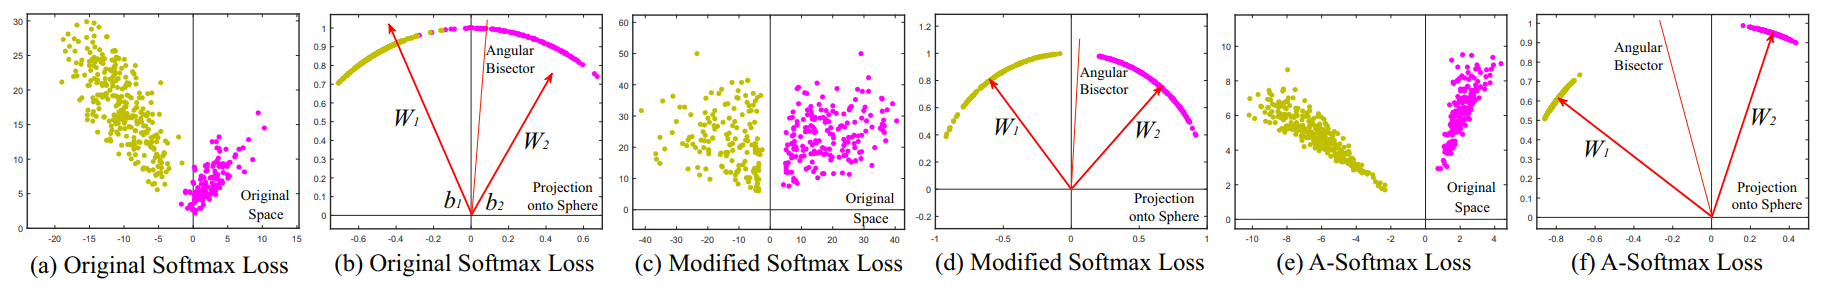
\includegraphics{images/closed_world/sphereface_whole.png}
     \caption{Функция потерь SphereFace сравнивает эмбеддинги по углу с вектором параметров классификатора \cite{liu2017sphereface}}
     \label{fig:sphereface}
 \end{figure}

 \begin{equation}
     \mathcal L_{modified} = - \frac{1}{n} \sum \limits_{i = 1}^{n} \log \frac{e^{\|x_i\| \cos (\theta_{y_i, i}) }}{e^{\|x_i\| \cos (\theta_{y_i, i})} + \sum_{j \neq y_i} e^{\|x_i\| \cos (\theta_{j, i})}}
 \end{equation}

 \begin{equation}
     \mathcal L_{ang} = - \frac{1}{n} \sum \limits_{i = 1}^{n} \log \frac{e^{\|x_i\| \psi (\theta_{y_i, i}) }}{e^{\|x_i\| \psi (\theta_{y_i, i})} + \sum_{j \neq y_i} e^{\|x_i\| \cos (\theta_{j, i})}}
 \end{equation}

 \textbf{CosFace, ArcFace}. Наконец, продолжая предыдущий метод, функции CosFace и ArcFace вводят в функцию потерь отступ, позволяющий разделять классы с некоторым зазором. Оптимальным вариантом является разделение прямой полосой с сферических координитах, что иллюстрирует \hyperref[fig:arcface]{Рисунке \ref*{fig:arcface}}.

 \begin{figure}[ht]
     \centering
     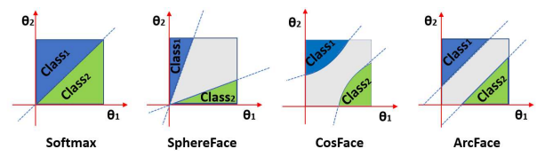
\includegraphics{images/closed_world/arcface.png}
     \caption{Функции CosFace и ArcFace позволяют строить зазор между эмбеддингами на сфере \cite{wang2018cosface}, \cite{deng2019arcface}}
     \label{fig:arcface}
 \end{figure}

 \begin{equation}
     \mathcal L_{cos} = - \frac{1}{n} \sum \limits_{i = 1}^{n} \log \frac{e^{s \left(  \cos (\theta_{y_i, i}) - m \right)}}{e^{s \left(  \cos (\theta_{y_i, i}) - m \right)} + \sum_{j \neq y_i} e^{s \cos (\theta_{j, i})}}
 \end{equation}

 \begin{equation}
     \mathcal L_{arc} = - \frac{1}{n} \sum \limits_{i = 1}^{n} \log \frac{e^{s \left(  \cos (\theta_{y_i, i} + m) \right)}}{e^{s \left(  \cos (\theta_{y_i, i} + m) \right)} + \sum_{j \neq y_i} e^{s \cos (\theta_{j, i})}}
 \end{equation}

 \subsection{Процесс обучения}

 Для некторых из представленных функций, в частности, для триплет-лосса, важной задачей является также подбор на каждой оптимизационной итерации наиболее сложных семплов датасета, обучение на которых внесет наибольший вклад в наполнение моделью информации о данных. Так, распространена техника \textit{hard-batch triplet mining} $-$ в качестве позитивного примера подается целевой кадр из батча, содержащий тот же объект, и представление которого наиболее отдалено от представления якорного. Аналогично, в качестве негативного подается наиболее близкий из остальных кадров. Кроме того, существуют техники, позволяющие моделировать более широкие взаимосвязи в данных для выявления оптимальных триплетов. Так, например, работа \cite{zeng2020hierarchical} объединяет метод hard-batch с иерархической кластеризацией семплов для выявления оптимальных троек кадров, \hyperref[fig:clusters]{Рисунок \ref*{fig:clusters}}:

 \begin{figure}[ht]
     \centering
     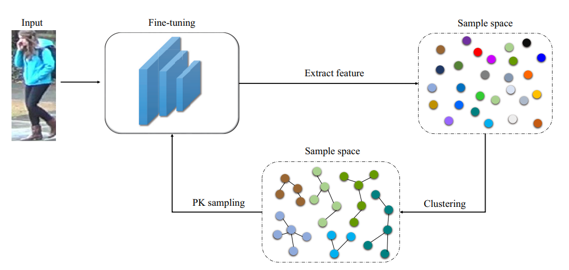
\includegraphics[width=0.7\textwidth]{images/closed_world/clusters.png}
     \caption{Иерархическая кластеризация в связке с hard-batch триплет mining \cite{zeng2020hierarchical}}
     \label{fig:clusters}
 \end{figure}


 \section{Оптимизация ранжирования}

 Благодаря метрическому обучению возможно получение ранжированных списков для объектов, поскольку функция расстояния позволяет упорядочить изображения в соответствии с похожестью. Однако данные списки могут быть улучшены, с помощью учета о взаимном положении объектов в ранжированных списках друг друга. Можно выделить две основные техники.

 \textbf{Ре-ранкинг}. Этот способ основан на том, что если два кадра соответствуют одному и тому же человеку, то каждый из них должен присутствовать в начале ранжированного списка другого. Поэтому данный метод позволяет удалить из списков некоторые неправильные ответы и добавить изначально ненайденные. Рассмотрим процедуру $k$-\textit{reciprocal re-ranking} \cite{zhong2017re}, проиллюстрированную на \hyperref[fig:reranking]{Рисунке \ref*{fig:reranking}}. На первом шаге для каждого кадра $x$ в ранжированном списке $r$ запроса $q$, имеющем размер $k$, строится свой ранжированный список размера $k$. Если $q$ в нем отсутствует, то $x$ удаляется из списка $r$. На втором шаге список $r$ пополняется константным количеством объектов из списков каждого оставшегося в $r$ кадра. Данная операция удаления-пополнения приводит к сокращению числа как ложно-положительных, так и ложно-отрицательных ответов.

 \begin{figure}[ht]
     \centering
     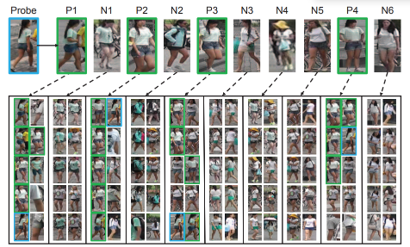
\includegraphics[width=0.7\textwidth]{images/closed_world/reranking.png}
     \caption{k-reciprocal re-ranking \cite{zhong2017re}}
     \label{fig:reranking}
 \end{figure}

 Полученные после этого алгоритма списки могут быть сравнены с помощью функции \textit{расстояния Джакарда}, которая строится на основе отношения размеров пересечения и объединения двух списков:

 \begin{equation}
     \mathcal R (q_i, k) = \{ x_j | (x \in r_i[:k]) \wedge (q \in r_j[:k]) \}
 \end{equation}

 \begin{equation}
     d_{J} (q_i, x_j) = 1 - \frac{| R(q_i, k) \cap R(x_j, k) |}{| R(q_i, k) \cup R(x_j, k)  |}
 \end{equation}

 \textbf{Слияние ранжированных списков}. Данный подход представляет собой метод ансамблирования нескольких моделей. Работа \cite{ye2016person} предлагает подход объединения ранжированных списков, основанный на усилении соотношений похожести между объектами в началах списков и непохожести $-$ в концах, \hyperref[fig:rank_fusion]{Рисунок \ref*{fig:rank_fusion}}:

 \begin{figure}[ht]
     \centering
     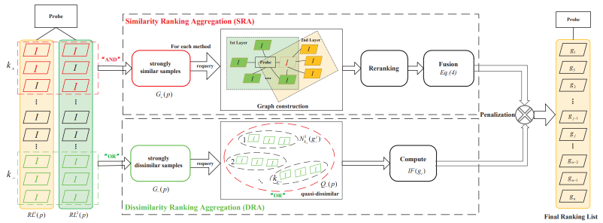
\includegraphics[width=0.7\textwidth]{images/closed_world/rank_fusion.png}
     \caption{Слияние ранжированных списков \cite{ye2016person}}
     \label{fig:rank_fusion}
 \end{figure}



 \endinput